\documentclass[conference]{IEEEtran}
\usepackage{times}
\usepackage[numbers]{natbib}
\usepackage{multicol}
\usepackage[bookmarks=true]{hyperref}
\hypersetup{hidelinks}
\usepackage{amssymb}
\usepackage{amsmath}
\usepackage{booktabs}
\usepackage{graphicx}
\usepackage{tikz}
\usetikzlibrary{positioning,arrows.meta}

\pdfinfo{
   /Author (Kangwei Sun)
   /Title (EmoMoconvq Final Report)
   /Subject (Physics-based motion generation)
   /Keywords (motion generation; emotion conditioning; physics-based)
}

\begin{document}

\title{EmoMoconvq: Parameter-Efficient Emotion Conditioning\\
for Physics-Based Motion Generation\\[3pt]
\large Final Project Report}

\author{Kangwei Sun 524531910006}

\maketitle

\begin{abstract}
We study whether MoConVQ~\cite{yao2023moconvq}, a frozen physics-based
text-to-motion model, can be retrofitted with discrete emotion control via
parameter-efficient fine-tuning. \textbf{EmoMoconvq} adds a 0.79M-parameter
emotion branch to T2M-MoConGPT's text features and distils supervision from
baseline responses to emotion-bearing text. In the strongest five-class
emotion-module-only variant, changing only the label increases mean pairwise
token disagreement from 0.560 under baseline sampling noise to 0.762
($1.36\!\times$; paired $t(49)=4.58$, $p=3.2\times10^{-5}$; bootstrap 95\%
ratio CI $[1.19,1.59]$). A separate focused three-class run obtains 39.3\%
token-classifier accuracy versus 33.3\% chance, although the classifier's
held-out validation accuracy is only 26.7\%, so we treat that result as
exploratory. After frozen physics decoding, six affective kinematic features
show no emotion effect (between-group ANOVA $p>0.7$; repeated-measures ANOVA
$p>0.39$; paired tests $p>0.26$). These results establish that the control
changes discrete outputs but do not establish that those changes encode
perceptible emotion. We present a frozen-decoder bottleneck as the leading
mechanistic hypothesis, discuss alternative explanations, and release code,
checkpoints, videos, and an interactive Gradio demo.
\end{abstract}

\IEEEpeerreviewmaketitle

\section{Introduction}
Physics-based motion generators are increasingly competitive with
kinematic-only models because they guarantee dynamic plausibility: the
generated motion is executed by an articulated character under contact and
gravity. The current state of the art, MoConVQ~\cite{yao2023moconvq},
generates physically simulated motion from text via a residual-VQ
representation combined with a GPT-style transformer (T2M-MoConGPT) and a
frozen physics tracking policy.

This expressive power comes with a control limitation: the model takes
unstructured natural-language text as its only conditioning signal. A
downstream system that wants to ``set the emotional state'' of an
animated character must phrase that state in text. This is brittle (the
exact wording matters; many emotion-action pairs are out-of-distribution)
and it conflates emotion with all other semantic content the text carries.

\textbf{Our question.}
Can we add a small \emph{discrete} emotion interface to MoConVQ's existing
text-to-motion stack, such that the same text prompt can be rendered in
different emotional styles by setting an explicit \texttt{emotion} flag?

\textbf{Our approach.}
We freeze the entire pretrained MoConVQ model and attach a small emotion
embedding module ($\sim 0.8$M trainable parameters) that perturbs the T5
text feature before it enters the temporal cross-attention layers
(\S\ref{sec:method}). Because no public dataset of emotion-labelled
physical motion exists in MoConVQ's character format, we adopt a
\emph{distillation} strategy: we run the baseline T2M-MoConGPT on text
that already contains explicit emotion adverbs (\textit{walks happily},
\textit{walks sadly}\ldots) to produce token sequences, then train
EmoMoconvq to reproduce those same token sequences from the \emph{stripped}
text plus the discrete emotion label (\S\ref{sec:distill}). Through three
progressive variants we tighten the design until the emotion label is, by
construction, the only input that distinguishes targets sharing a base caption
(\S\ref{sec:progress}).

\textbf{Our finding.}
Token-level evaluation (\S\ref{sec:tokeneval}) shows that the discrete label
changes the model output on held-out HumanML3D~\cite{guo2022generating}
captions: in the emotion-module-only model, variation is $1.36\!\times$
baseline stochasticity and is significant in a caption-paired test. A
separate three-class model obtains 39.3\% exploratory classifier accuracy
($33.3\%$ chance). However, kinematic tests on physically decoded motions
(\S\ref{sec:kineval}) find no emotion effect on six affective features. We
therefore investigate a \textbf{physics-decoder bottleneck}
(\S\ref{sec:discussion}) as the primary explanation, while retaining two
alternatives: the token differences may not be emotion-semantic, and the
selected kinematic features may miss perceptually relevant changes.

\textbf{Contributions.}
(i)~A clean, non-invasive emotion-conditioning architecture for MoConVQ
that is a strict parameter superset of the pretrained checkpoint.
(ii)~A reproducible three-stage distillation methodology that exposes the
emotion module's true capability without confounding text-memorisation.
(iii)~A token-level vs.\ motion-level decomposition that narrows where the
control signal is lost and exposes the limits of token-only evaluation.
(iv)~A carefully bounded negative result with a testable decoder-bottleneck
hypothesis and concrete follow-ups (decoder ablation and motion supervision).
(v)~A working Gradio interactive demo and 15-clip qualitative comparison
video set.

\section{Related Work}
\textbf{Physics-based motion generation.}
MoConVQ~\cite{yao2023moconvq} encodes motion into residual VQ tokens and
decodes them via a model-based RL policy that drives an ODE physics
simulator, trained on 23 hours of motion data. Its frozen encoder and
codebook make it well-suited for lightweight downstream adaptation,
which we exploit.

\textbf{Text-to-motion generation.}
T2M-GPT~\cite{zhang2023t2m} and MDM~\cite{tevet2022human} generate
kinematic motion from text using discrete transformers and diffusion
respectively. Both are trained on
HumanML3D~\cite{guo2022generating}, are not physics-based, and do not
expose an explicit emotion control.

\textbf{Style and emotion conditioning.}
ACTOR~\cite{petrovich2021action} conditions a transformer VAE on action
labels. Aberman et al.~\cite{aberman2020unpaired} learn motion style transfer
from an unpaired, style-labelled corpus, while 100STYLE~\cite{mason2022style}
provides 100 locomotion styles for real-time modelling. These systems still
depend on motion data whose skeleton and labels fit their training pipeline.
Our approach instead uses text-prompt distillation and leaves the pretrained
physics backbone unchanged.

\textbf{Parameter-efficient adaptation.}
We draw on the LoRA/adapter family~\cite{hu2022lora} in spirit. Our
emotion module is even lighter: $\sim$0.8M parameters with the rest of
the model frozen. Path~B of our experiments (\S\ref{sec:progress}) is
essentially a $\sim\!0.4\%$ adapter.

\section{Methodology and System Design}
\label{sec:method}

\subsection{System overview}
MoConVQ's text-to-motion pipeline has three frozen components: (1) a 1D
convolutional motion encoder + 8-layer residual VQ codebook
($N\!=\!512$, $d\!=\!768$); (2) T2M-MoConGPT, a dual transformer with a
12-layer temporal block and a 5-layer depth block predicting RVQ indices;
and (3) a deconvolutional decoder + mixture-of-experts tracking policy +
ODE physics simulator. We touch only the temporal transformer's input
(its T5 text feature) plus, optionally, its top few layers.

\subsection{Emotion embedding module}
Let $\mathcal{C}=\{\textit{neutral, happy, sad, angry, fearful}\}$ be the
5-class emotion set. We learn an embedding table
$E_e:\mathcal{C}\!\to\!\mathbb{R}^{d_e}$ ($d_e\!=\!512$) and a two-layer
MLP projection $\text{MLP}_{\text{proj}}:\mathbb{R}^{d_e}\!\to\!
\mathbb{R}^{d_{\text{T5}}}$ that lifts the emotion vector to the
1024-dimensional T5-large~\cite{raffel2020t5} feature space consumed by
cross-attention. The conditioning signal seen by every temporal block is
\begin{equation}
  f_{\text{cond}} \;=\; f_{\text{T5}}
  \;+\;\text{MLP}_{\text{proj}}\!\bigl(E_e(c)\bigr).
  \label{eq:fuse}
\end{equation}
The last linear of $\text{MLP}_{\text{proj}}$ is zero-initialised so that
$f_{\text{cond}}\!=\!f_{\text{T5}}$ at step 0 and the model degrades
gracefully to the pretrained baseline. The whole module is implemented
as a subclass of MoConVQ's transformer; the upstream source code is
unmodified. Loading the pretrained checkpoint into the subclass with
\texttt{strict=False} leaves exactly the 5 emotion tensors uninitialised
and produces no unexpected keys.

\subsection{Distillation training objective}
\label{sec:distill}
A complete public dataset of $(\text{text}, \text{emotion},
\text{MoConVQ-tokens})$ triples does not exist (\S\ref{sec:dataset-gap}).
We instead distil from the baseline:
\begin{enumerate}
\item Pick a set of \emph{base} captions $b$ that contain no emotion
words.
\item For each base $b$ and each emotion $e \in \mathcal{C}$, form the
\emph{augmented} caption $b^{(e)}$ by appending the canonical emotion
adverb (\textit{walks} $\to$ \textit{walks happily}).
\item Run the frozen baseline T2M-MoConGPT on each $b^{(e)}$ to obtain a
target token sequence $I^{(b,e)}$ and the corresponding quantised latent
sequence.
\item Train EmoMoconvq to predict $I^{(b,e)}$ given $(b, e)$ -- crucially,
the \emph{stripped} base text plus the emotion label, never the augmented
text.
\end{enumerate}
The training objective is the same per-token NLL loss as MoConGPT,
implemented from scratch (MoConVQ does not release training code).

Because $b$ is the same across all five emotions but the targets
$I^{(b,e)}$ differ, the text input alone cannot predict the target: the
model is \emph{forced} to use the discrete emotion label.

\subsection{Three progressive experimental variants}
\label{sec:progress}
We ran three increasingly tight variants to disentangle ``the module
learnt something'' from ``the module is the only thing that could have
learnt it''.

\textbf{v1 -- uncontrolled distillation, top-4 layers.} 463 unique
emotion-bearing captions filtered from HumanML3D, one emotion per
caption. The model can in principle memorise the text$\to$tokens map
purely from text features and ignore the emotion label. 47.3M trainable
parameters (24.3\% of the model).

\textbf{v2 -- 5-variant distillation, top-2 layers.} 100 base captions $\times$
5 emotions = 500 samples. Same base text, five different targets, so the
emotion label is the only distinguishing input. Train/val split is
\emph{base-stratified} so held-out captions are never seen in training.
24.0M trainable (12.4\%).

\textbf{Path B -- emotion-module only.} v2 dataset, but every temporal
layer is also frozen; only $E_e$ and $\text{MLP}_{\text{proj}}$ are
trainable. 0.79M trainable parameters (0.41\%).

\textbf{3-class D'.} v2 with the most challenging classes (\textit{sad},
\textit{angry}) removed -- the proposal's pre-registered fallback. 300
samples on $\{$neutral, happy, fearful$\}$; chance level 33.3\% (vs.\
20\%).

\section{Experiments and Evaluation}

\subsection{Datasets}
\label{sec:dataset-gap}

\textbf{Why distillation in the first place.} The original proposal
called for HumanML3D emotion-labelled motions plus CMU emotional-gait
sequences. Two practical blockers emerged. (1)~HumanML3D ships only text
annotations; the motion files require AMASS registration and large
download (40+~GB) plus a non-trivial SMPL$\to$MoConVQ retargeting
pipeline. (2)~MoConVQ uses a custom 22-joint skeleton with non-standard
joint names (\texttt{pelvis\_lowerback},
\texttt{rTorso\_Clavicle}, \ldots); its \texttt{BVHToTargetBase} loader
does name-matched pose copying, not real retargeting. We verified this
by attempting to load a public stylised-locomotion BVH from
100STYLE~\cite{mason2022style} (\textit{Angry/Angry\_BR.bvh}), which
failed immediately with
\texttt{KeyError: 'pelvis\_lowerback'}. A real retargeter would require
multi-week engineering, so we chose the distillation route, with full
disclosure of this scope change.

\textbf{Emotion-keyword corpus.} We scan HumanML3D's 23{,}384 training
captions ($\approx$70{,}000 caption lines) for any word from our
hand-curated emotion lexicon (e.g.\ \textit{happily, joyfully, sadly,
angrily, fearfully}\,\ldots). The resulting 463 caption--motion-id pairs
form the v1 corpus. Class counts are imbalanced (happy 126, sad 28,
angry 132, fearful 177); 229 of 463 are left/right mirror copies, so
HumanML3D's built-in mirror augmentation is already baked in.

\textbf{Distillation v2 corpus.} We sample 100 \emph{base} captions
from HumanML3D's training pool that satisfy: no emotion keyword present,
contains at least one motion-verb, length $\in [5, 25]$ words, motion id
not in the v1 set. For each base and each of the 5 emotions, the baseline
T2M-MoConGPT samples a target $(I, V)$ pair at a fixed seed. Output: 500
$(\text{base\_text}, \text{emotion}, I, V)$ triples; sequence length
distribution min 10, median 50, max 50, mean 40.4.

\subsection{Token-level compositional evaluation}
\label{sec:tokeneval}
We test compositional generalisation: does the trained EmoMoconvq actually
\emph{use} the discrete emotion label on captions that were not in
training? We sample 50 neutral test captions from the HumanML3D training
pool that (a) contain no emotion keyword and (b) have a motion id not in
any of our distillation sets.

For each test caption $c$, EmoMoconvq is run once per emotion at a fixed
seed, giving 5 outputs that differ \emph{only} in the discrete emotion
label. The baseline T2M-MoConGPT is run 5 times on the same $c$ with
different seeds, giving 5 outputs that differ only by sampling noise.
Two metrics:

\textbf{Separation ratio} = (mean pairwise token-disagreement among
EmoMoconvq's 5 outputs) $\div$ (mean pairwise disagreement among
baseline's 5 outputs). Values $>1.0$ mean the emotion knob produces
\emph{more} variation than baseline stochasticity.

For inference, we retain one emotion and one baseline disagreement score per
caption, compare them with a paired $t$-test, and bootstrap captions (50{,}000
resamples, fixed seed) to obtain a 95\% confidence interval for the ratio.
This paired design controls for caption-specific motion complexity.

\textbf{Classifier accuracy.} We train a small bi-GRU
(tokens $\to$ emotion) on the distillation dataset and apply it to
EmoMoconvq's compositional outputs. Per-class accuracy says whether the
model's outputs resemble the intended class in that learned token space.
Because this metric is meaningful only when the classifier generalises to
held-out distillation samples, we report its validation accuracy and treat
generation accuracy as exploratory when validation is at or below chance.

Figure~\ref{fig:progression} summarises both metrics across the four
experimental variants.

\begin{figure*}[t]
\centering
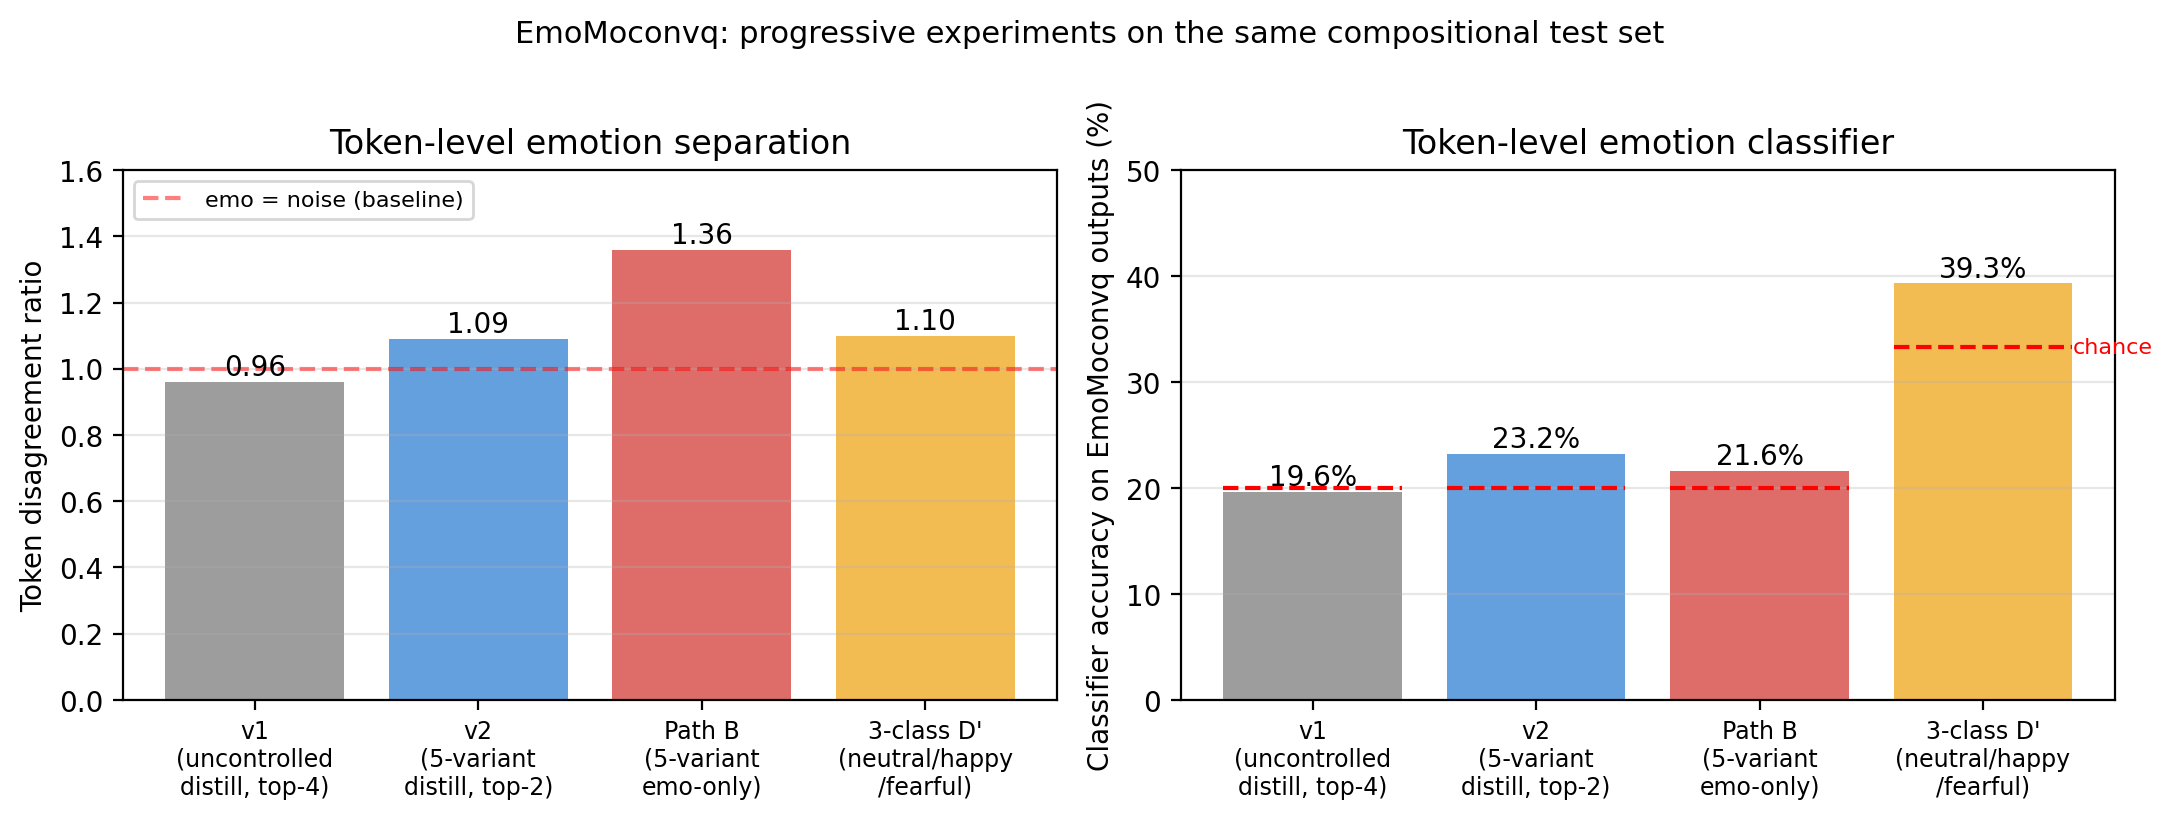
\includegraphics[width=0.95\textwidth]{fig_progression.png}
\caption{Token-level emotion separation across the four progressive
variants. Left: pairwise token disagreement caused by changing the emotion
label, normalised by baseline stochasticity. Right: descriptive classifier
accuracy on compositional-test outputs versus chance. The classifier panel
must be read with its held-out validation accuracy, discussed in the text.}
\label{fig:progression}
\end{figure*}

The trends are consistent at the disagreement level: v1 (loose,
large-capacity) is near baseline noise (ratio 0.96); v2 reaches 1.09; and
limiting capacity to the emotion module itself (Path~B) reaches 1.36. For
Path~B, mean disagreement is 0.762 versus 0.560 for baseline sampling. The
caption-paired difference is significant ($t(49)=4.58$,
$p=3.2\times10^{-5}$; Wilcoxon $p=3.9\times10^{-5}$), and the bootstrap 95\%
CI for the ratio is $[1.19,1.59]$. The emotion-embedding table moves by
$L_2$ norm 1.35 over training, about 8$\times$ the v1 shift. Thus the label
reliably changes token sequences, although disagreement alone does not show
that the changed tokens express the intended emotion.

\textbf{3-class focus.} In the focused setup
($\{$neutral, happy, fearful$\}$), generation accuracy is 39.3\% versus
33.3\% chance; per-class values are 30\% / 50\% / 38\%
(Fig.~\ref{fig:confusion}). However, the same classifier obtains only 26.7\%
on its held-out distillation split, below chance. The 39.3\% result is
therefore exploratory rather than confirmatory. Moreover, this model's token
separation ratio is 1.10, with a bootstrap 95\% CI $[0.90,1.35]$, so it does
not independently replicate Path~B's strong separation result.

\begin{figure}[t]
\centering
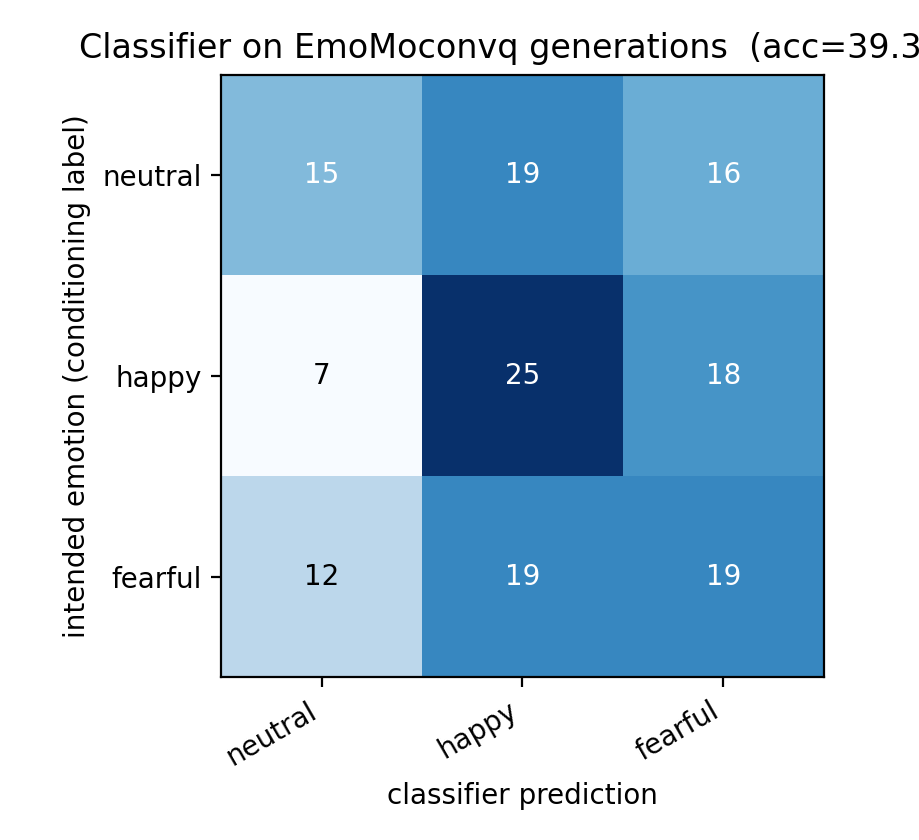
\includegraphics[width=0.85\columnwidth]{fig_confusion_3class.png}
\caption{Confusion matrix of the 3-class token classifier on compositional
outputs. Accuracy is 39.3\% (chance 33.3\%), but held-out classifier
validation is 26.7\%; consequently this matrix is descriptive, not evidence
of reliable emotion recognition.}
\label{fig:confusion}
\end{figure}

\subsection{Motion-level kinematic ANOVA}
\label{sec:kineval}
The above shows the \emph{tokens} differ. The next question is whether
the differences survive physics decoding. We ran EmoMoconvq through
MoConVQ's frozen physics decoder on 20 compositional test captions for
the 3 active emotions (60 simulated motions total) and computed six
features from the published affective-motion literature:
vertical energy (variance of root height; high $\Leftrightarrow$ bouncy),
mean root height, mean horizontal speed, foot-strike frequency, mean
trunk-lean angle, and arm-swing range.

Each feature was tested for a per-emotion effect with one-way ANOVA
(across-caption) and with paired analysis (within-caption: subtracting
the neutral baseline of the same caption). The result is unambiguous
(Table~\ref{tab:anova}, Fig.~\ref{fig:anova}):

\begin{table}[t]
\caption{One-way ANOVA: kinematic feature $\sim$ emotion label (20
captions $\times$ 3 emotions). No feature reaches the conventional
$p<0.05$ threshold; effect sizes $\eta^2 \le 0.011$.}
\label{tab:anova}
\centering
\small
\begin{tabular}{lrrr}
\toprule
Feature & $F$ & $p$ & $\eta^2$ \\
\midrule
vertical\_energy & 0.000 & 1.000 & 0.000 \\
avg\_height      & 0.036 & 0.965 & 0.001 \\
avg\_speed       & 0.178 & 0.838 & 0.006 \\
step\_freq       & 0.314 & 0.732 & 0.011 \\
lean\_angle      & 0.246 & 0.783 & 0.009 \\
arm\_swing       & 0.058 & 0.944 & 0.002 \\
\bottomrule
\end{tabular}
\end{table}

\begin{figure}[t]
\centering
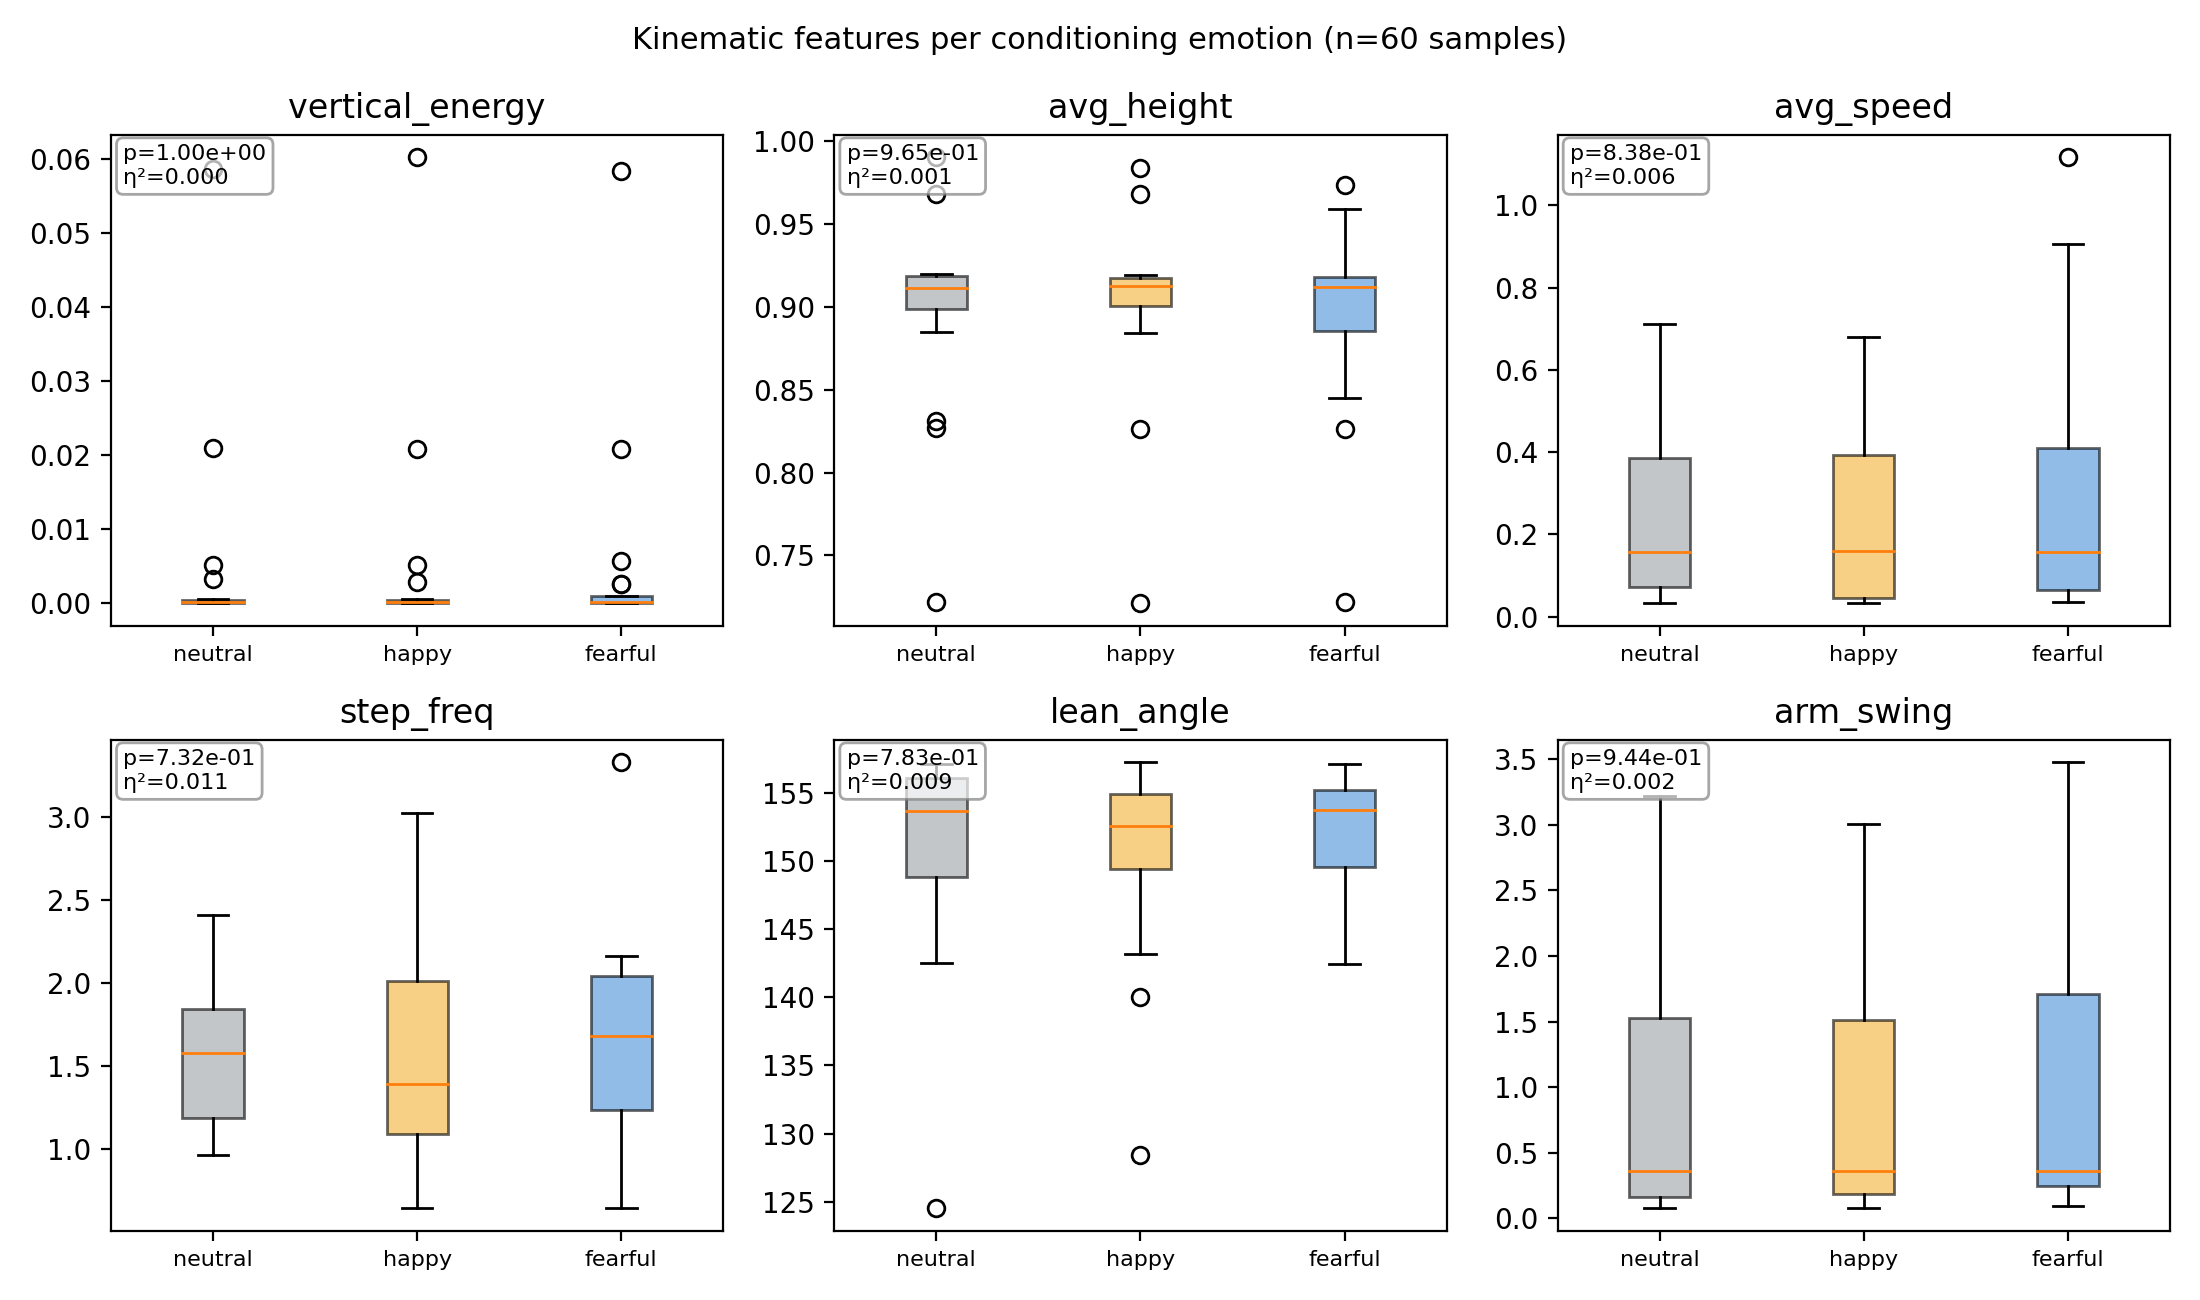
\includegraphics[width=\columnwidth]{fig_kinematic_anova.png}
\caption{Per-emotion distributions of the six affective kinematic
features over 20 compositional test captions. Boxes are essentially
indistinguishable across emotions; the embedded $p$-values are all
$>0.7$.}
\label{fig:anova}
\end{figure}

Within-caption analysis tells the same story (Fig.~\ref{fig:paired}). A
repeated-measures one-way ANOVA gives $p\in[0.391,0.823]$ and partial
$\eta^2\leq0.048$ across the six features. Paired $t$-tests against neutral
give $p\geq0.268$, and difference signs are split 40--60\% in either
direction. Under these predefined features and this sample size, we find no
systematic motion-level emotion effect.

\begin{figure}[t]
\centering
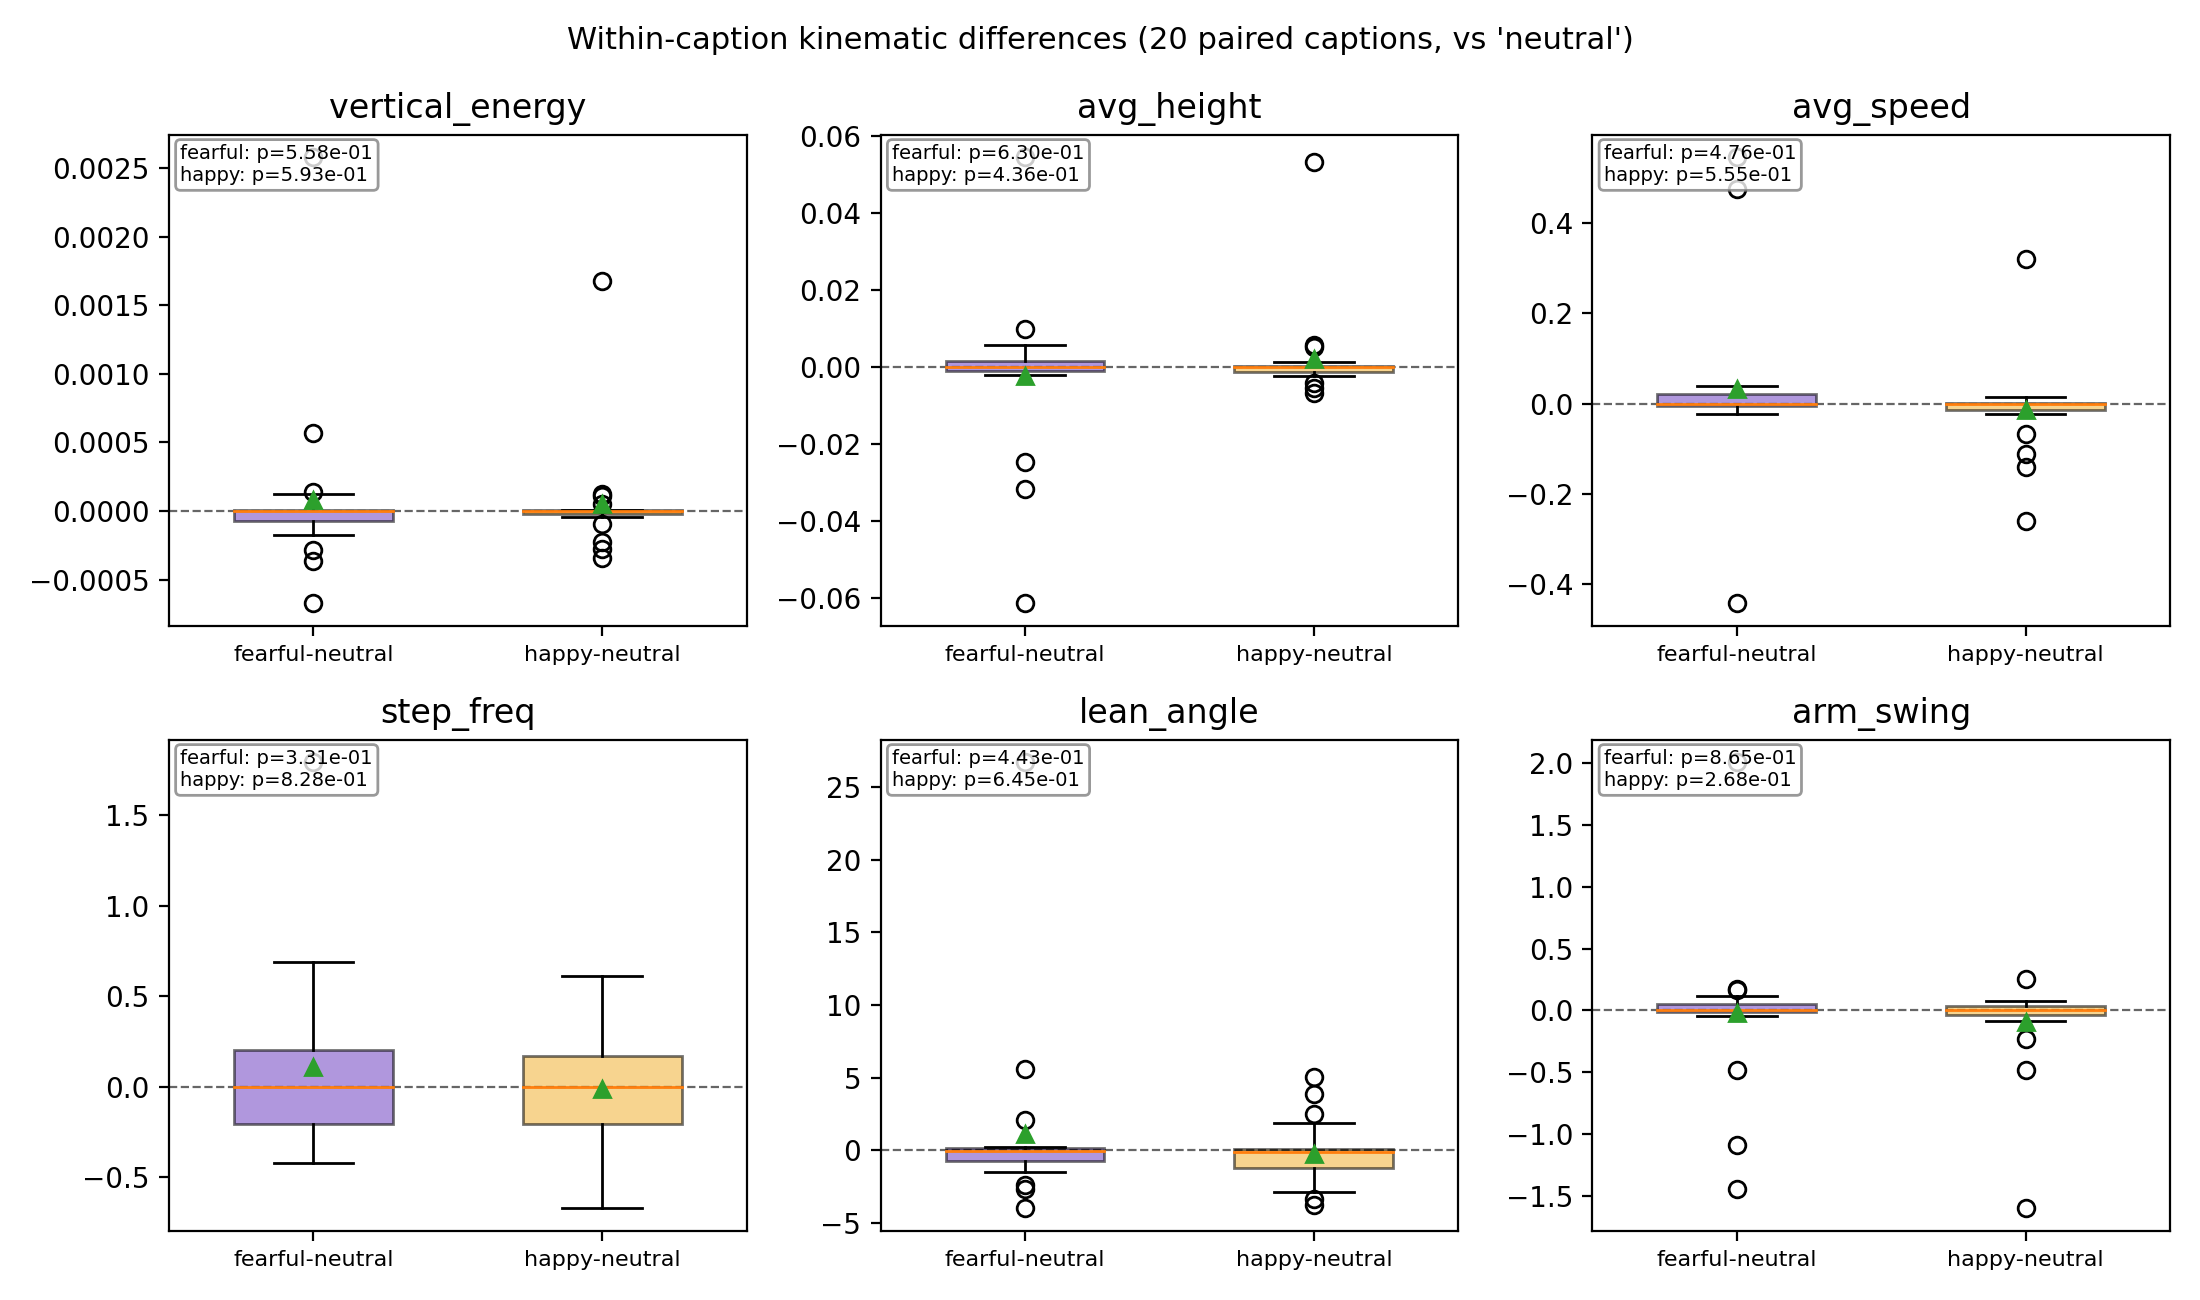
\includegraphics[width=\columnwidth]{fig_paired_diff.png}
\caption{Within-caption paired differences (vs.\ the same caption's
neutral baseline). Bars centred on zero; sign-consistency at $\approx$50\%
indicates no systematic emotion effect.}
\label{fig:paired}
\end{figure}

\subsection{Qualitative comparison \& interactive demo}
We render side-by-side comparison videos for 5 test captions $\times$ 3
emotions = 15 clips, decoded through MoConVQ's physics simulator,
visualised in Blender with a per-bone tracked skin geometry
(\texttt{render\_qualitative\_videos.py}). Some clips exhibit visible
trajectory or timing differences, but the differences are inconsistent
across captions and do not reliably map to the requested emotion. We did not
run a sufficiently powered, blinded user study; the videos are therefore
qualitative examples rather than perceptual evidence. They are released
alongside the code for independent inspection.

We also ship a Gradio web demo
(\texttt{Script/gradio\_demo.py}) that accepts a free-form text prompt,
an emotion label and a seed, and returns a downloadable BVH file
produced by EmoMoconvq through the physics simulator. The first request
loads the agent, T5-large, and our checkpoint ($\sim$2~min); subsequent
requests take $\sim$10~s each. This is a real, interactive, physics-based
emotion-conditioned generator.

\section{Results and Discussion}
\label{sec:discussion}

\subsection{Interpreting the token--motion gap}
The pattern in our results is:
\begin{itemize}
\item EmoMoconvq's emotion module \emph{is} trained: emotion-embedding
$L_2$-shift is large; the module receives non-trivial gradients.
\item Its \emph{token} outputs differ between conditioning labels and the
Path~B difference exceeds baseline noise ($1.36\!\times$ with a confidence
interval excluding 1).
\item The independent token classifier is not reliable enough to establish
that these differences encode emotion semantics.
\item Yet the \emph{decoded physical motion} is statistically
indistinguishable across emotions on six standard affective features.
\end{itemize}
Our leading hypothesis is that the frozen \textbf{physics-tracking policy}
acts as a regression toward its training distribution. MoConVQ's tracker was
trained, via model-based RL, to follow latent trajectories while maintaining
physical plausibility. A new conditioning branch can change upstream tokens
without providing the tracker motion-level supervision for the corresponding
style. The tracker may therefore map distinct upstream sequences to similar
joint torques, contacts, and centre-of-mass trajectories. We call this
candidate mechanism the \emph{decoder bottleneck}.

The current experiments do not causally localise the loss to the tracker.
Two alternatives remain. First, token disagreement may lie in code dimensions
that are redundant or unrelated to emotion before physics decoding. Second,
our six summary features may miss local timing, gesture, or trajectory cues
that a human observer could perceive. Distinguishing these explanations
requires an ablation that compares token, ConvVQ-latent, pre-simulation target
motion, and final simulated motion, plus a blinded perceptual study. Thus the
decoder bottleneck is a testable diagnosis, not a proven architectural law.

\subsection{Why the proposal's planned 60\% target was not reached}
The proposal targeted FID degradation $\le 0.5$, emotion-classifier
accuracy $\ge 60\%$, and $\ge 70\%$ user-study recognition. With the
observed token--motion gap, these targets were not reached. The 39.3\%
three-class generation score is exploratory because classifier validation is
below chance, and the motion-level tests are null. We report these outcomes
instead of presenting the descriptive score as successful emotion control.

\subsection{What this means for future work}
The decoder-bottleneck hypothesis motivates three concrete
follow-ups. Each requires substantial extra engineering that was beyond
the scope of this course project.

\textbf{(i) Decoder ablation and tracker adaptation.} First measure where
separation disappears by comparing ConvVQ latents, target poses, and simulated
poses. If the tracker is responsible, adapt it with policy-gradient updates or
a differentiable-physics surrogate while jointly training the emotion branch.
MoConVQ's released code does not expose this training path, so enabling it is
a non-trivial infrastructure project.

\textbf{(ii) Emotion-preservation loss in the tracking objective.}
Adding a term that penalises kinematic divergence from an
emotion-classifier's prediction. This requires a real, motion-data
emotion classifier, which in turn requires real emotion-labelled motion
data -- the same Path~C blocker we hit at evaluation time.

\textbf{(iii) End-to-end training on emotion-labelled physical motion.}
The proposal's original ambition. The barrier is the
MoConVQ-character retargeting problem we documented in
\S\ref{sec:dataset-gap}. Building a real retargeter (joint-topology
mapping, IK foot-contact correction, scale normalisation) for an
external emotion-mocap dataset is a multi-week engineering investment by
itself; we judged it out of scope for the remaining time budget after
fixing the data pipeline.

\section{Conclusion}
We built a clean, minimal, parameter-efficient emotion-conditioning
extension to a state-of-the-art physics-based text-to-motion model, and
tested it under progressively tighter experimental controls. The
emotion module verifiably changes token outputs beyond baseline sampling
noise in the strongest controlled variant. However, the classifier evidence
for emotion semantics is inconclusive, and the decoded motions show no
significant variation on six affective kinematic features. A frozen tracking
decoder is the leading explanation for this gap, but causal confirmation
requires intermediate-latent ablations and perceptual evaluation. The project
therefore contributes both a working conditioning system and a reproducible,
bounded negative result that identifies the next experiments needed for real
emotion-expressive physical motion.

\section*{Released artefacts}
Code, three trained EmoMoconvq checkpoints (v1, v2, 3-class), v1 \& v2
distillation datasets, 15 qualitative comparison videos, and the Gradio
demo are at
\url{https://github.com/Sunkw1224/EmoMoconvq}.

\bibliographystyle{plainnat}
\bibliography{references}

\end{document}
